% !TEX root = ../main.tex
\label{section:results}
\section{Results}

In this section, we compare the performance of the previously introduced models and methods and illustrate the results. They provide insight on the effects of incorporating knowledge about physical constraints and some limitations.

\subsection{Model architecture}
As described in the section \ref{ssec:network_architectures}, we first compare the three introduced network architectures. The performance of the models is displayed in Figure \ref{fig:models}.
\begin{figure}[H]
	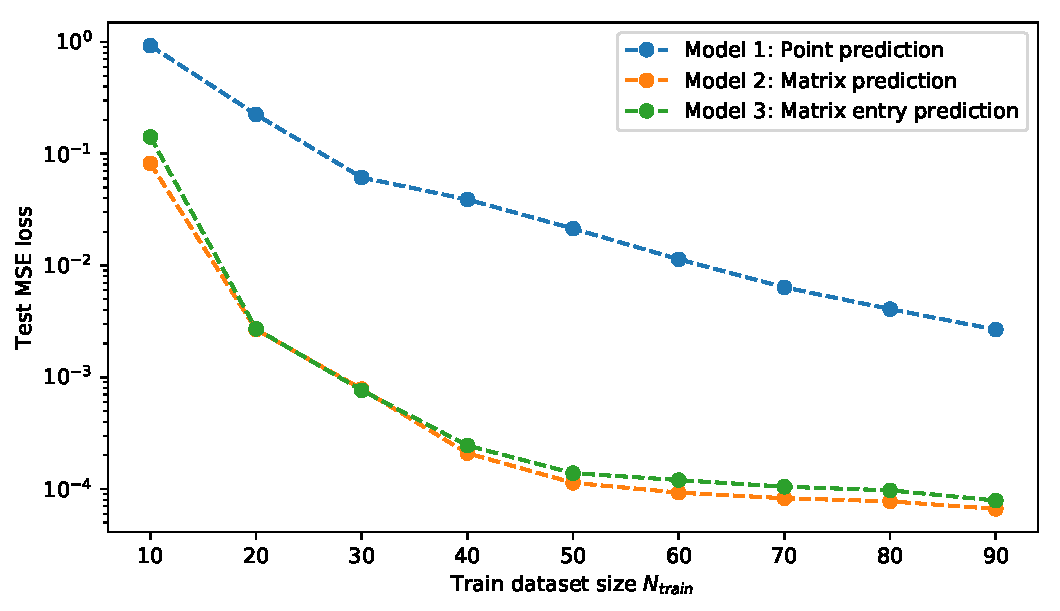
\includegraphics[width=\linewidth]{models}
	\caption{Different model architectures}
	\label{fig:models}
\end{figure}
We can see that while the difference between the behaviours of Model 2 and 3 is quite small, both of them perform significantly better than Model 1. Even when trained on 90 data points, Model 1 only achieves an error of $8\times 10^{-3}$, whereas Model 2 and 3 achieve a lower value of $2.7\times 10^{-3}$ with only 20 data points. This aligns with our expectations, since the latter two models already make use of the knowledge that a rotation can be represented as the multiplication of the point with a matrix that only depends on the rotation angle. Even though both matrix models perform well and almost the same for 20 and 30 data points, Model 2 finds a slightly better solution for most other amounts of training data. For example, with 10 data points, Model 2 achieves an error of $8.2\times 10^{-2}$, which is $41\%$ less than the performance of Model 3, which only reaches $1.4\times 10^{-1}$. The observed behaviour can be explained by looking at the structural difference of Model 2 and 3. Model 2 only uses one network with a single hidden layer that is fully connected with all output nodes which represent the rotation matrix entries. In contrast, Model 3 has an independent neural network for each matrix entry. As a consequence, the backpropagation in Model 3 for every network is done independently of the other neural networks. However, the matrix entries of the rotation matrix correlate heavily with each other, since the $\cos$ entries are exactly the same and the $\sin$ entires only differ in the sign. Therefore, trying to learn these entry values independently, as Model 3 does, constitutes a major disadvantage which leads to worse performance. \\
\indent Since Model 1 performs drastically worse than Model 2 and 3, we focus our experiments on the latter two models. Furthermore, due to time limitations, most of the following experiments are only carried out using Model 3. Future studies could check if the same behaviour occurs when applying the introduced methods to Model 2. Furthermore, since Model 3 already reaches a Test MSE Loss of less than $3\times10^{-3}$ with 20 training data points, but still performs poorly with only 10 points, the majority of the following analysis focuses on the interesting region of 10 to 20 as the size of the training dataset. \\
\indent However, we need to be careful not to attribute performance improvements to the incorporation of physical constraints if the same performance can also be achieved differently. Since both the Norm and the Determinant loss act as a form of regularisation, we need to check the effect of applying commonly used other types of regularisation. Hence, we apply L2-Regularisation with a wide range of different values for the weight decay. When conducting this experiment, we can observe no consistent improvement of the model's performance for any regularisation weight. The results can be looked up in the appendix in Figure \ref{fig:reg_weights}.

\subsection{Penalty method}
\subsubsection{Fixed physical loss weight}
\begin{figure}[h]
	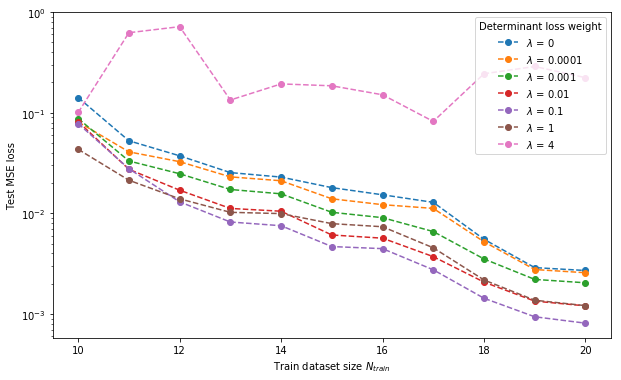
\includegraphics[width=\linewidth]{pnlty_det}
	\caption{Different weights $\lambda$ for $\mathcal{L}_{DET}$}
	\label{fig:pnlty_det}
\end{figure}
First, we apply the Penalty Method using a fixed weight $\lambda$ for the determinant physical loss $\mathcal{L}_{DET}$ and therefore only solve a single minimisation problem during the training process. The results obtained by this method performing $50\,000$ epochs on the 2D-Rotation problem using Model 3 are shown in Figure \ref{fig:pnlty_det}. When looking at these results, we immediatly observe the method's robustness to different weights of the physical loss, since small weights in a range of at least two orders of magnitude, namely $\lambda \in [0.01, 1]$, lead to significantly improved performance. For smaller values of $\lambda$, the test error converges to the one of $\lambda= 0$, whereas values of $\lambda > 1$ lead to a heavy focus on satisfying the physical constraint and thus leads to poor results compared to smaller values and $\lambda=0$.\\
\indent Moreover, we can see that the choice $\lambda = 0.1$ consistently yields a smaller error on the test dataset. It is also important to note that the performance improvement is significant. For example, with only 20 training data points, the physically trained model achieves a Test MSE Loss of $8\times10^{-4}$, whereas the model trained solely on the MSE Loss achieves only a value of $2.7\times10^{-3}$, thus reducing the error by more than $70\%$. \\
\indent Interestingly, utilising the penalty method leads to higher performance even for larger train datasets. This can be seen in Figure \ref{fig:pnlty_det_large} in the appendix, displaying the results of an experiment we conducted on a wider range including up to 100 training data points.\\
We observe similar qualitative behaviour when applying the method for the 3D-rotation, as displayed in Figure \ref{fig:pnlty_det_dim3} in the Appendix.\\
\begin{figure}[H]
	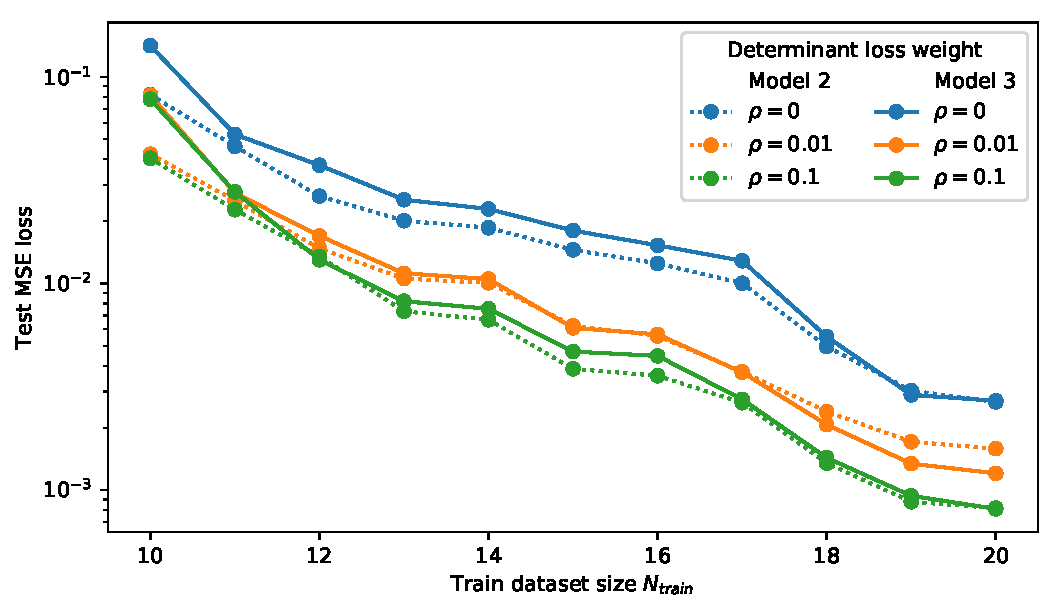
\includegraphics[width=\linewidth]{pnlty_det_models}
	\caption{Performance of the Fixed Penalty Method applied to Model 2 and Model 3 using different weights for the determinant loss.}
	\label{fig:pnlty_det_models}
\end{figure}
In order to check whether similar effects can be observed when using another model, we additionally apply the Fixed Penalty Method with the weights $\lambda = 0.01$ and $\lambda = 0.1$ to Model 2. The performance together with the one of Model 1 is depicted in Figure \ref{fig:pnlty_det_models}. When looking at these results, we can clearly see the same qualitative behaviour for the different physical loss weights compared to the baseline. For both models, applying the Penalty Method with the weights of both $\lambda = 0.01$ and $\lambda = 0.1$ improves performance significantly compared to not incorporating the physical constraints. These results provide a promising indication that the observed behaviour when applying the introduced methods to Model 3 also generalises to other model architectures. For this reason and due to time limitations, all of the following experiments are only carried out using Model 3. However, this assumption should be checked in future studies by applying the methods to Model 1 and Model 2.
\begin{figure}[H]
	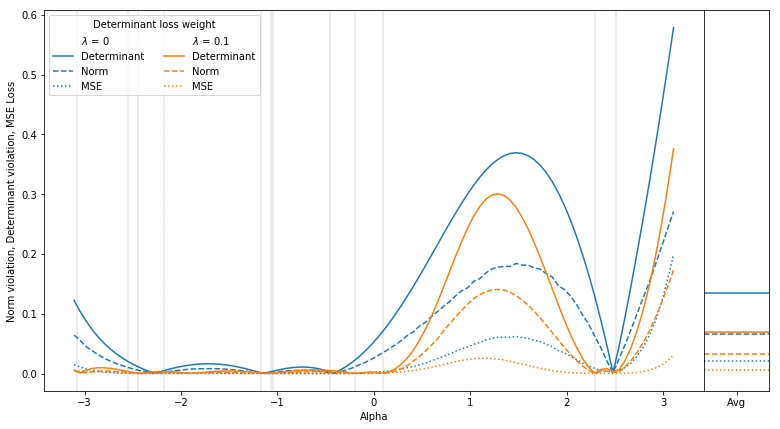
\includegraphics[width=\linewidth]{pnlty_det_analysis}
	\caption{Determinant and norm violations of predictions for $N_{train} = 12$. Gray vertical lines represent the angles of the training points.}
	\label{fig:pnlty_det_analysis}
\end{figure}
\indent Since we are not only interested in the overall test performance, but also how realistic the predictions are, we further need to analyse the physical feasability of the predictions. Figure \ref{fig:pnlty_det_analysis} shows the absolute difference of the determinant of the predicted rotation matrix and 1, the absolute difference of the norm of the predicted points and 1, and the test loss, all averaged across numerous points for each angle. First of all, we can see that the desired physical constraint is met perfectly at each training point, which already contributes to smaller overall errors in these regions. Even more important is the effect of the penalty method on predictions in areas where training data is sparse. An interesting region to analyse is the one for angles between $0.2$ and $2.2$, where not a single training data point exists. We can observe both smaller deviation of the determinant from one and smaller test error, meaning that the predictions are not only more realistic, but also closer to the true values.

\subsubsection{Increasing physical loss weight}
When analysing the version of the penalty method where we solve a series of minimisation problems with increasing weights $\lambda$ for $\mathcal{L}_{DET}$, we first have to discuss finding a good set of parameters. The parameters we need to determine for this method are the following:
\begin{itemize}
	\item Initial weight $\lambda_0 > 0$,
	\item Multiplier $\mu > 1$ which determines $\lambda_k = \mu^k\lambda_0$,
	\item Condition when to stop the current iteration,
	\item Number of iterations.
\end{itemize}
\begin{figure}[H]
	\centering
	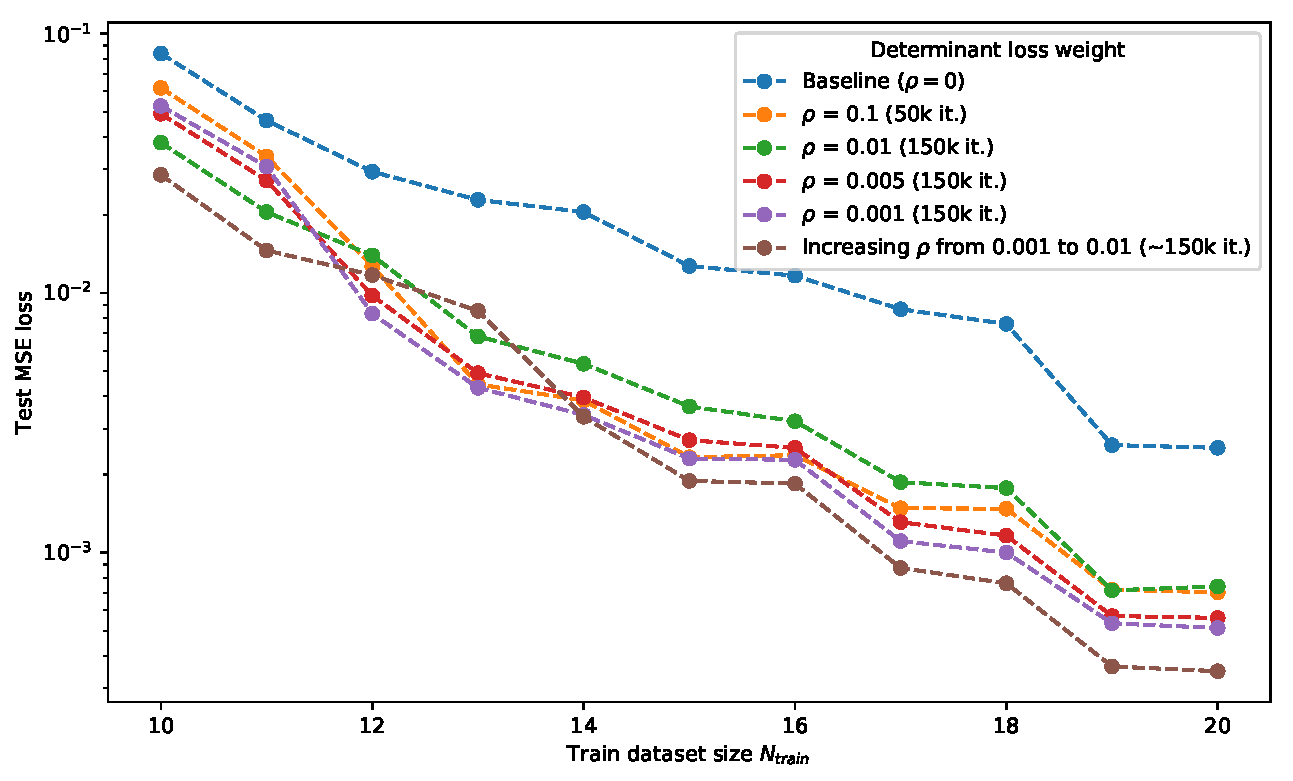
\includegraphics[width=\linewidth]{pnly_dyn}
	\caption{Different weights $\lambda$ for $\mathcal{L}_{DET}$ compared with dynamically increasing $\lambda$, averaged over 10 different training datasets.}
	\label{fig:pnly_dyn}
\end{figure}
In general, we can say that it is difficult to find a successful set of parameters, since we only have an intuition about the initial and last value of $\lambda$. We manually tried several different parameter sets, of which many led to much worse performance than the results shown above. However, we were able to increase the performance with the following values: We set $\lambda_0 = 10^{-3}$, $\mu = 1.05$, use 50 iterations and stop the k-th iteration once the norm of the gradient is smaller than $0.95^{k} 10^{-3}$. With this, we get an exponentially increasing series with a last weight value of $\lambda_{50} \approx 10^{-2}$. However, since solving a series of minimisation problems with the chosen parameters involves approximately $150\,000$ iterations, we also compare the results with using the fixed method for $150\,000$ iterations for different values taken by $\lambda$ during the dynamic training process. The results are illustrated in Figure \ref{fig:pnly_dyn}. We can see that the dynamic version outperforms the fixed Penalty Method by a significant margin for most training dataset sizes. For example, for 20 data points, the former achieves an error of $3.5\times 10^{-4}$, whereas the best fixed version only reaches twice the error of $7\times 10^{-4}$. Unfortunately, the improvement is not consistent and for 13 data points, the dynamic version only achieves $8.5 \times 10^{-3}$, whereas even the fixed Penalty Method with only $50\,000$ iterations already achieves with a value of $4.3 \times 10^{-3}$ almost half of this error.

As a summary, for the chosen parameters, the dynamic Penalty Method overall achieves higher performance than the fixed version. However, since it requires a multiple of the epochs needed by the fixed method and it is difficult to find a well performing set of parameters, we in general advise to use the simpler method using a fixed physical loss weight $\lambda$.

\subsection{Augmented Lagrangian Method}

We first apply the version which only computes a fixed number of epochs for each minimisation problem, and keep the weight $\mu$ of the physical loss $\mathcal{L}_{DET}$ constant. Thus, it differs from the first version of the Penalty Method only in having the additional linear constraint violation term. Note that for ALM, this weight needs to be chosen significantly smaller than for the Penalty Method depending on the constraint violation, since the linear term is much higher relative to the squared constraint violation term for small violation values. Still, it is similarly difficult to find a good set of parameters as it is for the second version of the Penalty Method. We achieved reasonable performance computing 30 iterations with $5\,000$ epochs each and a physical loss weight of $\mu = 0.01$. The Lagrangian multiplier estimates $\lambda$ are initially set to $0$ and updated according to equation \eqref{eq:alm_update}. Since we have one determinant constraint for every output, the Lagrangian multiplier estimate vector $\lambda$ contains $N_{train}$ values. The results are depicted in Figure \ref{fig:aug_lag} as "ALM fixed". In order to clearly extract the effect of incorporating ALM's core idea of including the linear constraint violation terms, we also include "ALM fixed (no linear)", which uses the same loss function, but omitting the linear terms. The results show that by using ALM with a good set of parameters, we can achieve even smaller error rates than the Penalty Method. For example, for 20 data points, the fixed ALM achieves an error of $3.9 \times 10^{-4}$, which is an improvement of $44\%$ compared to the error of $7 \times 10^{-4}$ of the Penalty Method, and also reduces the error by $24\%$ compared to its version omitting the linear terms, which reaches an error of $5.1 \times 10^{-4} $\\
\indent However, the improvements are not very consistent in the range between 10 and 15 training data points. Further, we have to note that the method also needs $150\,000$ epochs in total compared to the $50\,000$ epochs of the fixed Penalty Method in order to achieve comparable results. An example of the training and test loss after each iteration when applying the fixed ALM is shown in Figure \ref{fig:alm_fixed_training} in the Appendix. Since the Lagrangian multiplier estimates can be negative, we included the negative linear loss for the determinant as well.
\begin{figure}[H]
	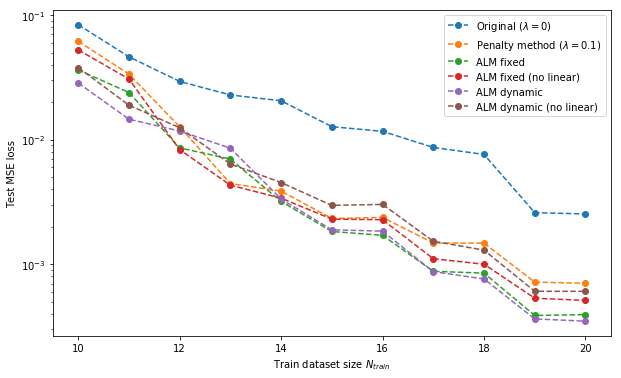
\includegraphics[width=\linewidth]{aug_lag}
	\caption{Comparison of ALM, Penalty Method and original training, averaged over 10 different random training datasets.}
	\label{fig:aug_lag}
\end{figure}
Furthermore, Figure \ref{fig:aug_lag} depicts the results of applying the second version of ALM, again including the comparison with the same computation without the linear term in the loss function. As described in section \ref{exp:alm}, we need to determine even more parameters than we do for the first version of ALM or the Penalty Method. This makes it especially difficult to find good parameters, and we need to mention that throughout the process of finding a good parameter set, we have tried many values that led to significantly worse performance than the original model which does not incorporate any physical constraints at all. To get reasonable results, we chose the following parameters: To begin with, we set $\mu_{0} = 10^{-3}$ and increased it by a factor of $1.05$ after each iteration. By computing 50 iterations, $\mu$ increases by approximately one order of magnitude. As before, the Lagrangian multiplier estimates are initially set to $0$ and updated according to equation \eqref{eq:alm_update}. The values for $\mu_k$ and $\lambda_k$ for a single run are depicted in the Appendix in Figure \ref{fig:mu_lambda_alm_dyn}. In order to make use of the proposed idea of setting the gradient threshold to a minimum of a fixed value and one dependent on the constraint violation, we set $\gamma_k = 0.95^k\,10^{-1}$ and $\epsilon_k = 0.95^k\,10^{-3}$. These values were chosen after analysing the constraint violation values during training and set such that $\epsilon_k$ and $\gamma_k ||c(x_k)||$ have approximately the same order of magnitude. The achieved results using these parameters are similiar to the fixed ALM results, and again achieve smaller error rates than the corresponding training omitting the linear term. For 20 training data points, it achieves an error of $3.5\times 10^{-4}$, which is close to the $3.9 \times 10^{-4}$ achieved by the fixed ALM. Overall, this is an improvement of $86\%$ compared to the original model which does not incorporate phyiscal constraints and thus only reaches an error of $2.5\times 10^{-3}$. However, also this version of ALM does not perform consistently better than the Penalty Method. Furthermore, it needs at least $150\,000$ and up to $300\,000$ epochs to achieve these results. Detailed numbers and statistics on the explained experiment are given in the Appendix (Table \ref{table_stats_10} - \ref{table_stats_20}).\\
\indent To understand the impact of ALM on how well the predictions align with the physical constraints, Figure \ref{fig:alm_det_analysis} depicts the absolute difference of the prediction norms and one, the absolute difference of the determinant of the predicted rotation matrix and one, and the corresponding MSE Loss. Note that results vary and Figure \ref{fig:alm_det_analysis} only depicts the values for 12 training data points and a single seed used to generate the training dataset.

\begin{figure}[]
	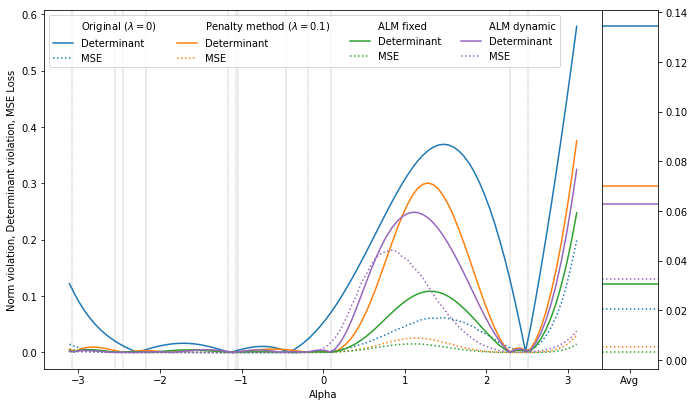
\includegraphics[width=\linewidth]{alm_det_analysis}
	\caption{Determinant and norm violations of predictions for $N_{train} = 12$. Gray vertical lines represent the angles of the training points.}
	\label{fig:alm_det_analysis}
\end{figure}

As expected knowing the statistical performance of the methods, the deviations from the physical constraints are significantly smaller when we apply one of the proposed methods compared to the original training. Similar to the Penalty Method, both versions of the Augmented Lagragian Method lead to no constraint violations at points where training data is present. While the fixed ALM in this case generalises the physical constraints significantly better than the Penalty Method, the dynamic version achieves only comparable results. Despite, an interesting observation is the high MSE Loss average of the dynamic ALM, which exceeds with a value of 0.033 the error of all other methods significantly. Even the original model achieves an overall average of the MSE Loss of only 0.021. However, this is only due to the performance in the range of angles between 0 and 2, for the extrapolation of angles higher than 2.5, it performs much better than the original model. This is the case even though the determinant in the difficult region is much closer to one than the determinant of the prediction of the original model. This indicates that the ALM focused too much on learning the determinant constraint, since it is able to generalise the determinant constraint only at cost of the performance of the predictions for this specific case. For three dimensions, we were not able to find a set of parameters leading to any improvements compared to the original model.\\
%\begin{figure}
%	\centering
%	\begin{subfigure}{.5\textwidth}
%		\centering
%		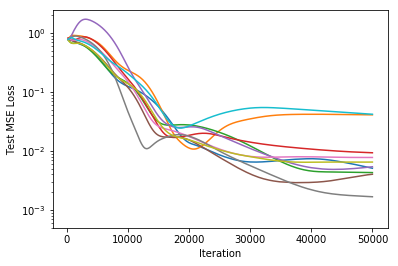
\includegraphics[width=\linewidth]{rand_test_pnlty}
%		\caption{Penalty method with $\lambda = 0.1$}
%	\end{subfigure}%
%	\begin{subfigure}{.5\textwidth}
%		\centering
%		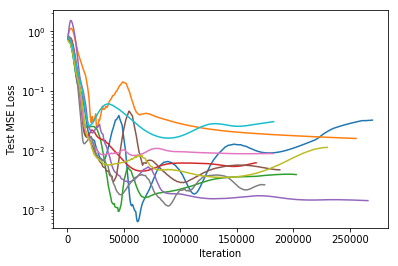
\includegraphics[width=\linewidth]{rand_test_alm_dyn}
%		\caption{Dynamic ALM}
%	\end{subfigure}
%	\caption{Test error throughout the training process for $N_{train} = 12$, each color represents a different training dataset. For example, the blue lines represent training for the random seed 1683.}
%	\label{fig:test_training}
%\end{figure}

%\begin{figure}
%	\centering
%	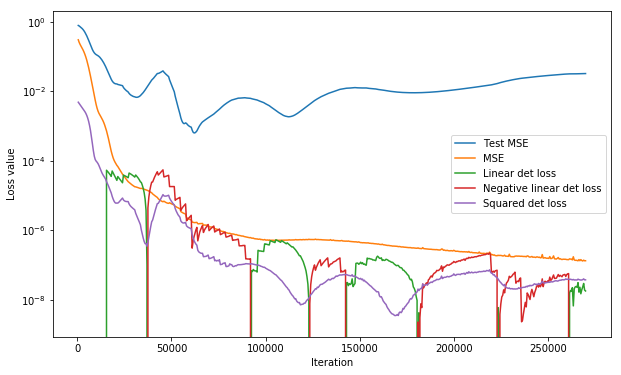
\includegraphics[width=.8\linewidth]{alm_1683_train}
%	\caption{ALM Training behaviour for $N_{train} = 12$ and the random seed 1683.}
%	\label{fig:alm_1683_train}
%\end{figure}
%\indent Furthermore, we want to point out that finding a good condition when to terminate the training process is difficult. The test performance throughout the training process for different randomly generated training datasets is depicted in Figure \ref{fig:test_training}. When comparing the performance of the Penalty Method (left) with the Dynamic ALM (right), we can instantly see much higher deviations when using the latter method. For example, the test performance colored in blue, representing training on the dataset created with the random seed 1683, reaches a test MSE Loss of less than $0.7\times 10^{-4}$, but only achieves an error of more than $3\times 10^{-2}$ when training has ended. In contrast, most of the test errors of using the Penalty Method converge and the following epochs only lead to slight overfitting. This in turn indicates the high potential of ALM as well. As we can see, the best performance achieved often exceeds the final performance significantly. This raises the question whether it is possible to find better conditions when to terminate the training process. In order to explore the training behaviour more deeply, we need to analyse the corresponding training loss. Since the previously discussed blue line depicting the model performance trained on the dataset created with seed 1683 shows the highest variance during training, we choose this example for a more detailed analysis. The corresponding training loss together with the test performance is depicted in Figure \ref{fig:alm_1683_train}. However, when looking at the training loss, there is no apparent sign indicating when training should have been terminated. Despite this fact, more sophisticated methods used to determine the hyperparameters of ALM and conditions when to terminate training might therefore lead to much higher improvements compared to what we achieve with the current parameters. 

\subsection{Failed experiments}

\subsubsection{Norm physical loss}
As we did for the physical constraint \eqref{eq:constraint_det} of the determinant being equal to one, we also tried to incorporate the constraint \eqref{eq:constraint_norm}, which says that the norm of the predicted point is supposed to be one. In contrast to what we expected and what we achieved incorporating the determinant constraint, we were not able to improve the performance of our model using the Penalty Method on the violation of the norm constraint. The results for different weights for $\mathcal{L}_{NORM}$ in the training loss for two and three dimensions are shown in Figure \ref{fig:pnlny_norm} in the Appendix.

\subsubsection{Physical Projection}
As explained in section \ref{sec:phys_proj}, we also tested an approach we call Physical Projection. We first applied it to the determinant constraint, thus scaling every predicted matrix with positive determinant according to equation \eqref{eq:norm_det}. Note that we detach the calculated scaling factor in order to not influence the gradient. Unfortunately, training using this procedure does not converge, an example is shown in Figure \ref{fig:normed_det_example} in the appendix.\\
\indent When applying the Physical Projection to the norm constraint, we again detach the calculated norm and only determine training loss and its gradient on the error between the normed prediction and the true point. As we can see in Figure \ref{fig:normed_pred} in the appendix, this approach does not improve the performance for either two or three dimensions. When further investigating the reason for this behaviour, we noticed that the norm of the predictions before scaling differs for regions that lack training data between them. The illustration in Figure \ref{fig:normed_pred_example} shows this behaviour well: For $-\pi < \alpha < 0.5$, the determinant of the predicted rotation matrix is only $\frac{1}{10}$ of the predicted determinant for $2 < \alpha < 3$. Even though predictions after the projection align with the physical constraints, it adds complexity to the problem, since the model can not make use of the rule that the determinant or norm is consistent accross all angles.







\clearpage

